\documentclass[10pt]{article}

\addtolength{\textwidth}{1.3in}
\addtolength{\oddsidemargin}{-.65in} %left margin
\addtolength{\evensidemargin}{-.65in}
\setlength{\textheight}{9in}
\setlength{\topmargin}{-.5in}
\setlength{\headheight}{0.0in}
\setlength{\footskip}{.375in}
\renewcommand{\baselinestretch}{1.0}
%\linespread{1.5}
\usepackage{setspace}
\doublespacing

\usepackage{titling}

\usepackage[pdftex]{graphicx}

\usepackage[usenames,dvipsnames]{color}
\usepackage{cite}
\usepackage{times, verbatim,bm,pifont,pdfsync}
\usepackage{caption}
\usepackage{subcaption}

\usepackage{tikz}
\tikzset{
% Two node styles for game trees: solid and hollow
solid node/.style={circle,draw,inner sep=1.5,fill=black},
hollow node/.style={circle,draw,inner sep=1.5,fill=white}
%non node/.style={circle,draw,inner sep=.1,fill=black}
}

% disables chapter, section and subsection numbering
%\setcounter{secnumdepth}{-1} 

\usepackage{amsbsy,amssymb, amsmath, amsthm, MnSymbol,bbding}
\usepackage[hang,flushmargin]{footmisc} 

\usepackage[pdftex,
bookmarks=true,
bookmarksnumbered=false,
pdfview=fitH,
bookmarksopen=true]{hyperref}

\newtheorem{definition}{Definition}
\newtheorem{theorem}{Theorem}
\newtheorem{lemma}{Lemma}
\newtheorem*{lemma*}{Lemma}
\newtheorem{corollary}{Corollary}
\newtheorem{assumption}{Assumption}
\newtheorem{fact}{Fact}
\newtheorem{result}{Result}

\newcommand{\ve}{\theta}
\newcommand{\ta}{\theta}
\newcommand{\ov}{\overline}
\newcommand{\un}{\underline}
\newcommand{\al}{\alpha}
\newcommand{\Ta}{\Theta}
\newcommand{\expect}{\mathbb{E}}
\newcommand{\Bt}{B(\bm{\tau^a})}
\newcommand{\bta}{\bm{\tau^a}}
\newcommand{\tad}{\tau^{ad}}
\newcommand{\bte}{\bm{\tau^E}}
\newcommand{\btn}{\bm{\tau^n}}
\newcommand{\ga}{\gamma}


\begin{document}
\title{\vskip-0.6in Temporary Trade Barriers: When Will They End?}%\protect\footnote{Formerly circulated under the title }}
\thanksmarkseries{alph}
\author{Kristy Buzard\thanks{Syracuse University, Economics Department, 110 Eggers Hall, Syracuse, NY 13244, USA. Ph: 315-443-4079. Fax: 315-443-3717. Email: kbuzard@syr.edu. http://faculty.maxwell.syr.edu/kbuzard.}} 
\date{\vskip-.1in \today}
\maketitle

\begin{center} {\bf Abstract} \end{center}

\begin{quote}
{Abstract

\textit{JEL classification:} D72, F13, F55 \\
\textit{Keywords:} temporary trade barriers, WTO, disputes, lobbying, political economy}
\end{quote}

\bigskip
\section{Introduction}

\begin{enumerate}
	\item How long do deviations from trade agreement tariffs last? 
  \item What are the determinants of renewals?
		\begin{itemize}
			\item They don't happen for \textit{no} reason at all
		\end{itemize}
\end{enumerate}

\vskip.2in
\begin{itemize}
	\item Temporary trade barriers have potential to be renewed
		\begin{itemize}
			\item For Anti-dumping (AD) duties, initial five year term, renewal for five years
			\item For Safeguards, four then four; much rarer than AD
		\end{itemize}
	\item Authorized by WTO
	\item Very little in the agreements to guide the process
		\begin{itemize}
			\item WTO litigation gives gov'ts a LOT of latitude
			\item Renewal decision determined by complex process including DOC, ITC, pressure via other political bodies.
		\end{itemize}
	\item In U.S., for AD:
		\begin{itemize}
			\item DOC initiates, determines whether dumping would continue
						\begin{itemize}
			\item Can renew AD duties
			\item Susceptible to influence of lobbying, perhaps both direct and indirect
			\item Modeled in reduced form
		\end{itemize}

			\item ITC determines whether injury would recur / continue
		\end{itemize}
\end{itemize}


\vskip.2in
The probability that an AD duty gets renewed

\begin{itemize}
	\item Increases in lobbying effort
	\item Decreases in the MFN tariff
	\item Is invariant to the trading partner's tariff
	\item Increases in the profitability of the import-competing sector
	\item Increases in the strength of the lobby
	\item May be concave in the AD duty
\end{itemize}

\subsection{Related Literature}
\textbf{WILL NEED MAJOR OVERHAUL}

Kara Reynold's ``Political Economy of Antidumping Reviews (Shushanik)

This work rests on the foundation of Grossman and Helpman's (1994) `Protection for Sale.' Two related papers `Trade Wars and Trade Talks' (Grossman and Helpman (1995b)) and `The Politics of Free-Trade Agreements' (Grossman and Helpman (1995a)) first employed the PFS approach in the study of trade agreements. The first considers ``Trade Wars'' and ``Trade Talks'' separately, whereas my approach views the ``Trade War'' as a crucial subgame. The model of preferential trade agreements (Grossman and Helpman (1995a)), although treating the government as a unitary actor, is closer to this approach.

Another related literature considers the impact of exogenously-determined political uncertainty on the potential for trade cooperation. These studies (e.g. Feenstra and Lewis (1991); Milner and Rosendorff (2001); Bagwell and Staiger (2005); Beshkar (2010); Horn, Maggi and Staiger (2010); Beshkar and Bond (2012)) derive various implications for the design of international trade agreements using a Baldwin (1987)-style government welfare function with exogenous shocks to the political-pressure parameter. 

Since trade policies are overwhelmingly determined in the context of trade agreements, it is useful to have a framework to bring together the endogenous political pressure of PFS-style modeling with the trade agreements approach. The government objective function introduced in this paper is intended to be a bridge between the two. This objective function starts from the Baldwin (1987) government objective function and adds flexibility: the weight the legislature places on profits is endogenous (PFS), potentially non-linear (Findlay and Wellisz 1982; Dixit, Grossman and Helpman 1997) and stochastic. Buzard (2016) is an example of how this modeling approach can be used to integrate  endogenous political activity and exogenous shocks into the analysis of questions regarding optimal trade agreement design.

Modeling the objective function so closely on the standard in the trade agreements literature allows for direct comparisons to the large body of work that studies exogenous shocks only, revealing cleanly the effects of the addition of endogenous lobbying. To preview, this model is closest to that of Bagwell and Staiger (2005), with two main changes: in place of their unitary government signing a trade agreement and having different preferences ex-ante and ex-post, this model has two branches of government with differing preferences, where the political economy weights of the legislature are determined endogenously.
		
Mansfield, Milner and Rosendorff (2000) study the impact of executive/legislative interactions on international agreements in the case of exogenously-determined preferences. They show that democracies trade more with each other because the domestic legislature only cooperates if the foreign government makes deep tariff cuts. Ethier (2002) treats the effect of a separation of powers between trade negotiators and the government officials who administer protection.

Milner and Rosendorff (1997) explore how uncertainty can affect trade policy and ratification failure when political preferences, and therefore uncertainty, are exogenous. In Le Breton and Salanie (2003), the lobby is uncertain about the preferences of a unitary decision maker. Le Breton and Zaporozhets (2007) replace the unitary decision maker with a legislature with multiple actors. In Song (2008), policy-making power is shared between an executive and a unitary legislature. The lobbies influence the preferences of the legislature in a context of unilateral policy making with no uncertainty, and Coates and Ludema (2001) study trade policy leadership with endogenous lobbying in the presence of political uncertainty with imperfect monitoring.


\section{The Model}
\label{sec:model}

\subsection{The Basic Setup}
\label{sec:basic}
I begin by describing the basic economic setting within which trade occurs. It is a three-good model with two countries: home (no asterisk) and foreign (asterisk). In each country, preferences are linear in good $N$, which is denoted the numeraire, while the demand functions for $X$ and $Y$ are assumed strictly decreasing and twice continuously differentiable. The demand functions for $X$ and $Y$ are taken to be identical and written $D(P_i)$ in home and $D(P_i^*)$ in foreign. $P_i$ ($P_i^*$) denotes the home (foreign) price of good $i \in \left\{N,X,Y\right\}$.

Good $N$ is produced with labor alone so that $Q_N = l_N$. I assume the aggregate labor supply is large enough to ensure that the output of good $N$ is enough to guarantee balanced trade. The supply functions for good $X$ are $Q_X(P_X)$ and $Q_X^*(P_X^*)$ and are assumed strictly increasing and twice continuously differentiable for all prices that elicit positive supply. For any such $P_X$, I assume $Q_X^*(P_X) > Q_X(P_X)$ so that the home country is a net importer of good $X$. The production structure for good $Y$ is symmetric, with demand and supply such that the economy is separable in goods $X$ and $Y$. The production of goods $X$ and $Y$ requires labor and a sector-specific factor that is available in inelastic supply and is non-tradable so that the income of owners of the specific factors is tied to the price of the good in whose production their factor is used. 

For simplicity, I assume each government's only trade policy instrument is a specific tariff on its import-competing good: the home country levies a tariff $\tau$ on good $X$ while the foreign country applies a tariff $\tau^*$ to good $Y$. Local prices are then $P_X = P_X^W + \tau$, $P_X^* = P_X^W$, $P_Y = P_Y^W$ and $P_Y^* = P_Y^W + \tau^*$ where a $W$ superscript indicates world prices. Equilibrium prices are determined by the market clearing conditions
$$M_X(P_X)= D(P_X)-Q_X(P_X) = Q_X^*(P_X^*) - D(P_X^*) = E_X^*(P_X^*)$$
$$E_Y(P_Y)=Q_Y(P_Y)-D(P_Y) = D(P_Y^*)-Q_Y^*(P_Y) = M_Y^*(P_Y^*)$$
where e.g. $M_X$ are home-county imports and $E_X^*$ are foreign exports of good $X$. The price of the numeraire is equal to one in both countries and on the world market.

$P_X^W$ and $P_Y^W$ are decreasing in $\tau$ and $\tau^*$ respectively, while $P_X$ and $P_Y^*$ are increasing in the respective domestic tariff. This gives rise to a terms-of-trade externality. Profits in a sector are increasing in the price of its good and also in the domestic tariff. This fact, combined with the assumptions on specific factor ownership, motivates political activity by the import-competing lobby.

In the home country, there is a government agency that has the power to renew (or not) antidumping duties. To focus attention on protectionist political forces, highlight the model's central mechanisms and minimize the number of actors that must be modeled, we assume that only the import-competing industry is politically-organized and that it is represented by a single lobbying organization.\footnote{The model extends easily to the case of multiple lobbies.\label{fn:lobby}} Policy-makers and lobbyists in the foreign country are assumed to be passive.

\textbf{REVISE EXTENSIVE FORM}

\begin{figure}
	\begin{center}
		\begin{comment}
\documentclass[10pt]{article}

\addtolength{\textwidth}{1.3in}
\addtolength{\oddsidemargin}{-.65in} %left margin
\addtolength{\evensidemargin}{-.65in}
\setlength{\textheight}{9in}
\setlength{\topmargin}{-.5in}
\setlength{\headheight}{0.0in}
\setlength{\footskip}{.375in}
\renewcommand{\baselinestretch}{1.0}
\usepackage{setspace}
\doublespacing

\usepackage{titling}

\usepackage[pdftex]{graphicx}

\usepackage[usenames,dvipsnames]{color}
\usepackage{cite}
\usepackage{times, verbatim,bm,pifont,pdfsync}
\usepackage{caption}
\usepackage{subcaption}

\usepackage{tikz}

% disables chapter, section and subsection numbering
\setcounter{secnumdepth}{-1} 

\usepackage{amsbsy,amssymb, amsmath, amsthm, MnSymbol,bbding}
\usepackage[hang,flushmargin]{footmisc} 

\usepackage[pdftex,
bookmarks=true,
bookmarksnumbered=false,
pdfview=fitH,
bookmarksopen=true]{hyperref}


\newcommand{\ta}{\theta}
\newcommand{\al}{\alpha}
\newcommand{\Ta}{\Theta}
\newcommand{\expect}{\mathbb{E}}
\newcommand{\Bt}{B(\bm{\tau^a})}
\newcommand{\bta}{\bm{\tau^a}}
\newcommand{\bte}{\bm{\tau^E}}
\newcommand{\btn}{\bm{\tau^n}}
\newcommand{\ga}{\gamma}


\begin{document}
\end{comment}

\tikzset{
% Two node styles for game trees: solid and hollow
solid node/.style={circle,draw,inner sep=1.5,fill=black},
hollow node/.style={circle,draw,inner sep=1.5,fill=white}
%non node/.style={circle,draw,inner sep=.1,fill=black}
}
\begin{tikzpicture}[scale=1.5,font=\footnotesize, grow=right]
% Specify spacing for each level of the tree
\tikzstyle{level 1}=[level distance=10mm,sibling distance=8mm]
\tikzstyle{level 2}=[level distance=8mm,sibling distance=8mm]
% The Tree
\node(0)[solid node,label=above:{$E,E^*$}]{} 
child{node(1)[solid node,label=below:{$0$}]{}}
child{[white] node(2)[solid node,xshift=12,label=above:{L}]{}  
	child{[black] node(4)[solid node,label=below:{$0$}]{}}
	child{[white] node(5)[hollow node,xshift=12]{} 
	 child[sibling distance=11mm]{[black] node(22)[solid node]{}  }
	 child[sibling distance=11mm]{[black] node(23)[hollow node]{}  
		child[sibling distance=8mm]{[black] node(7)[solid node,label=below:{$-\infty$}]{}}
		child[sibling distance=8mm]{[white] node(8)[solid node,xshift=12]{}  
			child[sibling distance=10mm]{[black] node(10)[solid node]{}  }
			child[sibling distance=10mm]{[black] node(12)[solid node]{}  
				child[sibling distance=5mm]{[black] node(13)[solid node,label=below:{$0$}]{}}
				child{[white] node(15)[solid node,xshift=7]{} 
					child[sibling distance=5mm]{[black] node(19)[solid node,label=below:{$-\infty$}]{}}
					child{[white] node(21)[solid node,xshift=7]{} 
						child[sibling distance=5mm]{[black] node(16)[solid node,label=below:{$0$}]{} }
						child{[white] node(18)[hollow node,xshift=12,label=left:{}]{}  }
						child[sibling distance=5mm]{[black] node(17)[solid node,label=above:{$\infty$}]{} }
						edge from parent node[black, xshift=16]{$\ta_n$} 
						}
					child[sibling distance=5mm]{[black] node(21)[solid node,label=above:{$\infty$}]{} }
					edge from parent node[black, xshift=15]{$e_n$} 
				}
				child[sibling distance=5mm]{[black] node(14)[solid node,label=above:{$\infty$}]{} }
				}
			edge from parent node[black, xshift=20]{$\ta_b$} 
			}
		child[sibling distance=8mm]{[black] node(9)[solid node,label=above:{$\infty$}]{} }
		}
	 edge from parent node[black, xshift=20]{$e_b$} 	
	 }
	child{[black] node(6)[solid node,label=above:{$\infty$}]{}}
	edge from parent node[black, xshift=23]{$\bta$} 
	}
child{node(3)[solid node,label=above:{$\infty$}]{}
}
;
% information set
    \draw[solid,bend right](1)to(3);
		\draw[solid,bend right](4)to(6);
		\draw[solid,bend right](7)to(9);
		\draw[solid,bend right](13)to(14);
		\draw[solid,bend right](16)to(17);
		\draw[solid,bend right](19)to(21);
% labels
		\node[above,xshift=3,yshift=5]at(2){$L$}; 
		\node[above,xshift=1,yshift=5]at(23){$N$}; 
		\node[above,xshift=3,yshift=5]at(5){$N$}; 
		\node[above,xshift=6,yshift=5]at(8){$Leg$}; 
		\node[above,xshift=5,yshift=5]at(12){$L$};
		\node[above,xshift=13,yshift=-17]at(21){$Leg$}; 
		\node[above,xshift=7,yshift=5]at(15){$N$}; 
		\node[left, xshift=-2]at(18){$\tau^n$}; 
		\node[below left,yshift=-12]at(12){Break}; 
		\node[below left,yshift=4]at(10){Abide}; 
		\draw[solid](5)circle(.05cm);
		\draw[solid](0)circle(.15cm);
		\node[right]at (10) {$W_E\left(\bta\right),$};
		\node[right,yshift=-10]at (10) {$\pi\left(\tau^a\right)-e_b,$};
		\node[right,yshift=-20]at (10) {$W_{ML}\left(\ga(e_b,\ta_b),\bta\right)$};
		\node[right]at (18) {$W_E\left(\btn\right),$};
		\node[right,yshift=-10]at (18) {$\pi\left(\tau^n\right)-e_b -e_n,$};
		\node[right,yshift=-20]at (18) {$W_{ML}\left(\ga(e_n,\ta_n),\btn\right)$};
		\node[right,yshift=-5]at (22) {$W_E\left(\bta\right),$};
		\node[right,yshift=-15]at (22) {$\pi\left(\tau^a\right)-e_b,$};
		\node[right,yshift=-25]at (22) {$W_{ML}\left(\ga(e_b,\ta_b),\bta\right)$};
		\node[below left,xshift=-4,yshift=8]at(23){Opp.}; 
		\node[below left,xshift=-4,yshift=-10]at(23){(o)}; 
		\node[below left,xshift=-3,yshift=7]at(22){No opp.}; 
		\node[below left,xshift=6,yshift=20]at(22){(1-o)}; 
\end{tikzpicture}

%\end{document}
	\end{center}
	\caption{Extensive Form\label{fig:ext}}
\end{figure}

Figure~\ref{fig:ext} illustrates the timing of the game. Taking the trade-agreement tariffs $\bta = \left(\tau^a,\tau^{*a}\right)$\footnote{I use the convention throughout of representing a vector of tariffs for both countries $(\tau,\tau^*)$ as a single bold $\bm{\tau}$.} and the antidumping duty level $\tad$ as given, the import-competing firms jointly attempt to persuade the government agency to renew the antidumping duties by choice of lobbying effort $e$. 

After this, uncertainty about the government agency's preferences is resolved. 

Lobby must be able to trigger the original AD duty
\begin{itemize}
	\item \textit{Can} think of non-adherence to MFN as eqm path dispute
	\item It could be justified, not motivated by politics/rent-seeking
	\item But still, firms lobby for duties they don't get
\end{itemize}


\vskip.1in
So what's the uncertainty about?

\begin{itemize}
	\item Strength of evidence
	\item Probability foreign will retaliate or initiate dispute (indirect)
	\item $G$'s valuation of harm to industry, e.g. how politically important is industry?
	\item Uncertainty could be, in part, about how mobile labor is (Kishore)
\end{itemize}

All players simultaneously observe the realization of the random variable $\ta$ that represents this uncertainty. The political stage concludes with the agency making a choice to renew the antidumping duties or let them expire. In the event that the antidumping duties expire, the home country's trade policy reverts to the trade agreement tariff $\tau^a$. Finally, producers and consumers make their decisions.


\subsection{Preferences}
\label{sec:pref}
With foreign not active in setting policy and the structure the economy symmetric and fully separable, I focus on the home country and the $X$-sector, which is the only politically active sector. The government agency's welfare is given by
\begin{equation}
  W_{\mathit{G}} = \mathit{CS}_X(\tau) + \ga(e,\ve) \cdot \pi_X(\tau) + \mathit{CS}_Y(\tau^*) + \pi_Y(\tau^*) + \mathit{TR}(\tau)
  \label{eq:ml}
\end{equation}
where $\mathit{CS}$ is consumer surplus, $\pi$ are profits, $\ga(e,\ta)$ is the weight placed on profits in the import-competing industry, and $\mathit{TR}$ is tariff revenue.\footnote{Labor income $l$ could also be included in government welfare. I omit it because its inclusion alters none of the results and only serves to complicate the exposition.} I model the decisions of the government agency as being taken by a median actor with the weight the median actor places on import-competing industry profits affected by the level of lobbying effort $e$ and a random variable $\ta$. I make the following assumptions on $\ga(e,\ta)$:

\begin{assumption}
  $\ga(e,\ta)$ is increasing and concave in $e$ for every $\ta \in \Theta$.
  \label{as:ga_c}
\end{assumption}

\begin{assumption}
  $\ga(e,\ta)$ is increasing in $\ta$.
  \label{as:ga_ta}
\end{assumption}

\begin{assumption}
  $\ta$ is uniformly distributed on some $\Theta=\left[\underline{\ta},\overline{\ta}\right]$.
  \label{as:ta}
\end{assumption}

Assumption~\ref{as:ga_c} means that the government agency favors the import-competing industry more the higher is its lobbying effort, but that there are diminishing returns to lobbying activity. It rules out higher effort making lower weights more likely and that the structure of uncertainty changes with increasing effort so that higher weights become more likely at an accelerating pace. Assumption~\ref{as:ga_ta} simply provides for an intuitive labeling so that larger realizations of $\ta$ increase the value of the political economy weight.

Given its expectations and the government agency's preferences, the home lobby chooses its lobbying effort $e$ to maximize the welfare function:
\begin{equation}
  \expect \left[U_L \right] = \Pr\left[ \text{AD Renewal} \right]  \pi_X(\tau^{\mathit{ad}}) +\left\{1-\Pr\left[ \text{AD Renewal}\right]\right\} \ \pi_X(\tau^a) - e
  \label{eq:lv}
\end{equation}
where $\pi(\cdot)$ is the current-period profit. 


\subsection{Information and Equilibrium Selection}
\label{sec:info}

\textbf{NOT SURE AT ALL ABOUT THESE FEATURES; it's not a two-country model}

I examine a simple class of equilibria that have three key features. First, information about political uncertainty is symmetric. However, in line with the literature, I assume the lobby's contribution is not observable to the foreign legislature. Thus the influence of one country's lobby on the other country's legislature occurs only through the tariffs selected.\footnote{cfr. Grossman and Helpman (1995b), page 685.} Since players in the same country can take advantage of more information than those who are in different countries, the solution concept is perfect public equilibrium (PPE).

Second, whenever there is a possibility of multiple equilibria, I focus on the one that maximizes the executives' welfare. Since I assume the executives are social welfare maximizers, this selection criterion puts results in terms of the maximal level of trade policy cooperation that is possible. It also allows the question of whether governments use trade agreements as political commitment devices to be answered in a straightforward way.

Finally, I assume that an external authority can ensure enforcement of the agreement.


\section{Main Results}
\label{sec:main}

The government agency will renew the antidumping duty if the median actor's utility from the antidumping duty is higher than his utility from the trade agreement tariffs, i.e. if
\begin{equation}
  W_G(\tad,\tau^{*a},\ga(e,\ve)) > W_G\left(\bta,\ga(e,\ve)\right)
  \label{eq:lwcg}
\end{equation}
  
The outcome of the decision on whether or not to renew the antidumping duties is not known to \textit{any} player until the uncertainty over the identity of the median governmental actor is resolved at the moment the decision is made. I represent the probability that antidumping duties are renewed as:
\begin{multline}
  r(e,\bta,\tad) = \expect_{\ga|e} \bm{1} [ W_G(\tad,\tau^{*a},\ga(e,\ve)) > W_G\left(\bta,\ga(e,\ve)\right) ] \\ = \Pr [ W_G(\tad,\tau^{*a},\ga(e,\ve)) > W_G\left(\bta,\ga(e,\ve)\right) | e]
  \label{eq:b}
\end{multline}

The lobby chooses its level of effort as a function of the trade agreement tariffs and the antidumping duties, given the implications of that choice on the government agency's probability of renewing the duties. In effect, the lobby maximizes probability-weighted profits net of effort:
\[
  \max_{e} r(e,\bta,\tad) \pi(\tau^{ad}) + [1 - r(e,\bta,\tad)] \pi(\tau^a) - e
\]
The first order condition shows that the lobby balances the cost of an extra dollar of expenditure with the higher profits from anti-dumping duties weighted by the increase in the probability of receiving the extension of the antidumping duties:
\begin{equation}
	\frac{\partial r(e,\bta,\tad)}{\partial e} \left[ \pi(\tau^{ad})  - \pi(\tau^a) \right] = 1 
	\label{eq:lobbyfoc}
\end{equation}
Result~\ref{res:bincC} below and the fact that antidumping duties are necessarily larger than trade agreement tariffs ensure the second order condition. To guarantee an interior solution, we need
  \begin{equation}
	  \frac{\partial r(0,\bta,\tad)}{\partial e} \left[ \pi(\tau^{ad}) - \pi(\tau^a) \right] > 1.
		\label{ine:lobint}	
  \end{equation}
It may be that either the antidumping duty is too low or the marginal impact of the first lobbying dollar is too small for it to be in the lobby's interest to exert effort. The main results of the paper only hold when the marginal impact of the first lobbying dollar on the renewal probability is sufficiently high to make engaging in the political process worthwhile for the lobby.
  
I represent the total probability that the antidumping duties will be renewed as $R(\bta,\tad)=r(e(\bta,\tad),\bta,\tad)$ where $e(\bta,\tad)$ is the best response function implicit in Equation \ref{eq:lobbyfoc}, the lobby's first order condition. We next examine the question of how the total renewal probability varies as both a direct and indirect function of both trade agreement tariffs and antidumping duties, as well as industry profitability and political influence. Each result must take into account that the variable of interest can have both a direct effect on the renewal probability and an indirect effect through lobbying incentives.


\bigskip
\subsection{Home Trade Agreement Tariffs}
\label{sec:home}

Let's look first at the direct effect of changing $\tau^a$ on the renewal probability. For any effort level $e$, when the trade agreement tariff is very low, only a small set of realizations of $\ta$ associated with the lowest values of $\ga(e,\ta)$ will lead to the antidumping duties being re-approved, implying a high renewal probability. As the trade agreement tariff rises, larger values of $\ga(e,\ta)$ are consistent with approving the trade agreement, so the set of $\ta$'s that lead to trade agreement approval is larger. That is, the renewal probability decreases as $\tau^a$ increases. 

\begin{lemma}
  The direct effect of the home trade agreement tariff on the probability the government renews the antidumping duty is negative. \hyperlink{Pr_leg_a}{Proof}
  \label{res:leg_a}
\end{lemma}

All proofs are in the Appendix. 

The indirect effect is made up of two parts: the impact of raising the home trade agreement tariff on lobbying effort, and the impact of lobbying effort on the renewal probability. Starting with the question of how lobbying effort varies in the home trade agreement tariff, notice that raising the trade agreement tariffs decreases the benefit of a renewal in the trade agreement by raising trade agreement profits. This implies that lobbying effort is lower when trade agreement tariffs are higher.

\begin{lemma}
  Lobbying effort is weakly decreasing in trade agreement tariffs. \hyperlink{Pr_lobby}{Proof}
  \label{res:lobby}
\end{lemma}

Turning to the second component of the indirect effect, it's useful to note that lobbying affects only the weight the government agency places on the profits of the import-competing industry. These profits are higher under antidumping duties than under the trade agreement tariff. Assumption~\ref{as:ga_c} implies that the government becomes more favorably inclined---albeit at a decreasing rate---toward the higher antidumping duties and associated profits as lobbying increases and thus more likely to renew the antidumping duties. 

\begin{lemma}
  The probability that the government agency renews the antidumping duties is increasing and concave in lobbying effort $\left(\text{i.e. } \frac{\partial r}{\partial e} \geq 0, \ \frac{\partial^2 r}{\partial e^2} \leq 0  \right)$. \hyperlink{Pr_bincC}{Proof}
  \label{res:bincC}
\end{lemma}

Result~\ref{res:bcomB} combines the direct and indirect effects to get the total effect of trade agreement tariffs on the renewal probability.

\begin{result}
	The total probability that the antidumping duties will be renewed is decreasing in $\tau^a$ (i.e. $\frac{\partial R(\bta,\tad)}{\partial  \tau^a} \leq 0$). \hyperlink{Pr_bcomB}{Proof}
	\label{res:bcomB}
\end{result}

\noindent When $\tau^a$ is higher, the government agency becomes less likely to renew the antidumping duties, for three reasons. First, the government prefers a higher domestic tariff (Lemma~\ref{res:leg_a}); second, the higher tariff discourages lobbying, reducing $R(\bta,\tad)$ indirectly (Lemma~\ref{res:lobby}); and finally, the lower lobbying effort directly reduces the government's preferred tariff further (Lemma~\ref{res:bincC}).


\bigskip
\subsection{Foreign Trade Agreement Tariffs}
\label{sec:foreign}

Turning to the effect of the foreign trade agreement tariffs on the probability that the antidumping duties will be renewed, it is perhaps not surprising that there is no effect:
\begin{result}
  The total probability that the antidumping duties will be renewed is constant in the foreign trade agreement tariff. \hyperlink{Pr_astar}{Proof}
  \label{res:leg_astar}
\end{result}

Because the duties are a unilateral policy that we presume here are permissable under WTO rules, the decision to renew the duties or not does not change the level of the tariff applied by the foreign trading partner. That is, there is no incentive in terms of reciprocal treatment to deter the home government from renewing the duties.


\bigskip
\subsection{Antidumping Duties}
\label{sec:tad}


\begin{lemma}
  The direct effect of an increase in the antidumping duty on the probability the government renews the antidumping duties is negative. \hyperlink{Pr_tad_dir}{Proof}
  \label{res:tad_dir}
\end{lemma}


\begin{lemma}
  Lobbying effort is weakly decreasing in the antidumping duties. \hyperlink{Pr_tad_indir}{Proof}
  \label{res:tad_indir}
\end{lemma}


\begin{result}
	The total probability that the antidumping duties will be renewed is decreasing in level of the antidumping duties $\tad$. (i.e. $\frac{\partial R(\bta,\tad)}{\partial \tad} \leq 0$). \hyperlink{Pr_tad_total}{Proof}
	\label{res:tad_total}
\end{result}




\bigskip
\subsection{Political Weighting Function}
\label{sec:gamma}

We next examine the weight the median decision-maker places on the profits of the import-competing sector. The value of the political weight $\ga(e,\ta)$ is endogenous to many of the decisions underpinning the equilibrium, but here we examine the effect of an exogenous shift in the weighting function itself, $\ga(\cdot,\ta)$. We start again with the direct effect:

\begin{lemma}
  The direct effect of exogenous positive shifts in the political weighting function $\ga(\cdot,\ta)$ on the probability the government renews the antidumping duty is positive. \hyperlink{Pr_ga_dir}{Proof}
	  \label{res:ga_dir}
\end{lemma}

In accordance with intuition, if there is a shift in the political weighting function so that the government agency weights the profits of the import-competing sector more heavily for a given amount of lobbying effort....


\begin{lemma}
  Lobbying effort is weakly increasing in the uniform exogenous positive shifts of the political weighting function. \hyperlink{Pr_ga_indir}{Proof}
  \label{res:ga_indir}
\end{lemma}


\begin{result}
	The total probability that the antidumping duties will be renewed is increasing in $\ga$. (i.e. $\frac{\partial R(\bta,\tad)}{\partial  \ga(\cdot)} \geq 0$). \hyperlink{Pr_ga_total}{Proof}
	\label{res:ga_total}
\end{result}


%This translates in a straightforward way to an impact on the trade agreement tariff.

%\begin{corollary}
%  Exogenous positive shifts in the political weighting function $\ga(e)$ lead to higher trade agreement tariffs, \emph{ceteris paribus}.
%  \label{cor:tg}
%\end{corollary}

%\noindent This makes sense given that an upward shift in the political weighting function in effect means that the lobby becomes more powerful---that is, it has a larger impact on the median legislator for a given level of effort. This is why the minimum effort level required to break the trade agreement is reduced, and therefore why the trade agreement tariff must be increased: when the lobby has to pay less to break the agreement for any given tariff level, the agreement must be made more agreeable to the lobby.


\subsection{Profitability of Import Competing Sector}
\label{sec:pi}


\begin{lemma}
  The direct effect of a change in the import competing sector's profitability on the probability the government renews the antidumping duty has the same sign as the change in the gap between profits under antidumping duties and profits under the trade agreement tariff. \hyperlink{Pr_pi_dir}{Proof}
  \label{res:pi_dir}
\end{lemma}


\begin{lemma}
  The effect of a change in the import competing sector's profitability on lobbying effort has the same sign as the change in the gap between profits under antidumping duties and profits under the trade agreement tariff. \hyperlink{Pr_pi_indir}{Proof}
  \label{res:pi_indir}
\end{lemma}

Notes:
\begin{itemize}
	\item For $\frac{\partial R}{\partial \pi} \geq 0$, need the return from lobbying to increase with increase in $\pi$ AND
	\item government marginal benefit from protection to increase with $\pi$
\end{itemize}

\vskip.2in
\begin{itemize}
	\item Profit function convex $\Rightarrow$ also quasiconvex
	\item But hit it with the right increasing monotone transformation and $\frac{\partial }{\partial \pi(\cdot)} \left[\pi_X(\tad) - \pi_X(\tau^a) \right]$ can go either way
	\item This is about how the differences change (CARDINAL)
\end{itemize}


\begin{result}
	The total probability that the antidumping duties will be renewed increases (decreases) when there is an increase (decrease) in the gap between profits under antidumping duties and profits under the trade agreement tariff. \hyperlink{Pr_pi_total}{Proof}
	\label{res:pi_total}
\end{result}







\section{Conclusion}
\label{sec:concl}
			
			Future Work

\begin{itemize}
	\item Comparative static on uncertainty measure
	\item Empirical work
	\item Extend model to include initial decision to grant protection.
		\begin{itemize}
			\item Explain variation in a lobby's incentives between original application of AD and renewal
			\item Lobby's choice between investing in productive vs. rent-seeking behavior while protected
			\item Need to have first stage (Jee-Hyeong, Gary Lyn)
		\begin{itemize}
			\item Look at Park and Blonigen (Jee-Hyeong)
			\item Cost differential for firms to get initial duty vs. renewal?
			\item Some firms choose not to pursue renewal when DOC contacts them 30-days before (Sasha)
		\end{itemize}
	\item Lobbying effort may be endogenous: if prob. of success is lower, maybe it's not worth providing effort (Mostafa)
		\end{itemize}
\end{itemize}




\section{Appendix}
\label{sec:appendix}
\noindent \textbf{\hypertarget{Pr_leg_a}{Proof of Lemma~\ref{res:leg_a}}}:

Substituting from Equation~\ref{eq:ml}, Equation~\ref{eq:b} can be re-written as
\begin{multline}  
  r(e,\bta,\tad) = \Pr [ \mathit{CS}_X(\tad) + \ga(e,\ve) \cdot \pi_X(\tad) + \mathit{CS}_Y(\tau^{*a}) + \pi_Y(\tau^{*a}) + \mathit{TR}(\tad) >  \\ \mathit{CS}_X(\tau^a) + \ga(e,\ve) \cdot \pi_X(\tau^a) + \mathit{CS}_Y(\tau^{*a}) + \pi_Y(\tau^{*a}) + \mathit{TR}(\tau^a) ]
\end{multline}
Rearranging, we have $r(e_b,\bta,\tad) = $
\begin{multline}  
  \textstyle \Pr \Big[ \frac{\mathit{CS}_X(\tad) + \pi_X(\tad) + \mathit{CS}_Y(\tau^{*a}) + \pi_Y(\tau^{*a}) + \mathit{TR}(\tad)  -\mathit{CS}_X(\tau^a) - \pi_X(\tau^a) - \mathit{CS}_Y(\tau^{*a}) - \pi_Y(\tau^{*a}) - \mathit{TR}(\tau^a)}{\pi_X(\tau^a) - \pi_X(\tad)} + 1 \\ \textstyle < \ga(e,\ve) \Big]
  \label{eq:b_ex}
\end{multline}

The effect on the renewal probability is determined by the sign of the derivative of the left hand side of the inequality in Expression~\ref{eq:b_ex} with respect to $\tau^a$; to show that the renewal probability is decreasing in $\tau^a$, I must demonstrate that this derivative is positive. Labeling the left hand side of the inequality in Expression~\ref{eq:b_ex} $Z(\bta,\tad)$ and the numerator of that expression $ZN(\bta,\tad)$, the derivative of this quantity with respect to $\tau^{a}$ is 
\begin{equation}
  \frac{\left(\pi_X(\tad) - \pi_X(\tau^a)\right)\left(\frac{\partial \mathit{CS}_X(\tau^{a})}{\partial \tau^{a}} + \frac{\partial \pi_X(\tau^a)}{\partial \tau^{a}} + \frac{\partial \mathit{TR}(\tau^{a})}{\partial \tau^{a}}\right) - ZN(\bta,\tad) \frac{\partial \pi_X(\tau^a)}{\partial \tau^a}}{\left(\pi_X(\tau^a) - \pi_X(\tad)\right)^2}.
  \label{appex:a}
\end{equation}

\noindent $\left(\pi_X(\tad) - \pi_X(\tau^a)\right)$ is always positive. Because the optimal unilateral tariff for large welfare-maximizing governments is positive (call it $\tau^O$), $\left(\frac{\partial \mathit{CS}_X(\tau^{a})}{\partial \tau^{a}} + \frac{\partial \pi_X(\tau^a)}{\partial \tau^{a}} + \frac{\partial \mathit{TR}(\tau^{a})}{\partial \tau^{a}}\right)$ is increasing up to $\tau^O$ and decreasing above it. Thus the first summand is increasing up until $\tau^O$ and decreasing thereafter.

It is also positive over the remaining $(\tau^O,\tad)$. To see this, add $\left(\tilde{\Gamma} - 1 \right) \frac{\partial \pi_X(\tau^a)}{\partial \tau^a} \left(\pi_X(\tad) - \pi_X(\tau^a)\right)$ to the first summand and subtract it from the second. For any particular value of $\tilde{\tau}^a$, one can choose the $\tilde{\Gamma}$ weight that would make $\tilde{\tau}^a$ the preferred unilateral tariff; this makes the derivative in the first summand zero. Having subtracted the same quantity from the second summand modifies the welfare difference in the second summand to be maximized at $\tilde{\tau}^a$ so that this term is always positive (inclusive of the leading negative sign).

Since the denominator is a squared term of a strictly positive quantity, the expression in Equation~\ref{appex:a} is positive for all $\tau^{a}$.  $\hfill\blacksquare$


\vskip.4in
\noindent \textbf{\hypertarget{Pr_lobby}{Proof of Lemma~\ref{res:lobby}}}:\\
Proof is via the Implicit Function Theorem using the lobby's first order condition, Equation~\ref{eq:lobbyfoc}, referred to here as $FOC_L$.
  \[
		\frac{\partial e}{\partial \tau^a} = - \frac{\frac{\partial FOC_L}{\partial \tau^a}}{\frac{\partial FOC_L}{\partial e}} = \frac{ \frac{\partial r}{\partial e} \frac{\partial \pi(\tau^a)}{\partial \tau^a} - \frac{\partial^2 r}{\partial e \partial \tau^a} \left[ \pi(\tad) - \pi(\tau^a) \right]}{\frac{\partial^2 r}{\partial e^2} \left[ \pi(\tad) - \pi(\tau^a) \right]}
	\]
Beginning with the denominator: $\tad > \tau^a$ and $\pi(\cdot)$ is increasing in $\tau$ so the expression is brackets is positive. $\frac{\partial^2 r}{\partial e^2}$ is negative by Result~\ref{res:bincC}, so the denominator is negative.

Turning to the numerator: $\frac{\partial r}{\partial e}$ is positive and $\frac{\partial \pi(\tau^a)}{\partial \tau^a}$ is positive by construction so the first term is positive. 

We can rewrite $\frac{\partial r(e,\bta,\tad)}{\partial  \tau^a} = -\frac{\partial F_\ga (Z(\bta,\tad))}{\partial \tau^a} = -\frac{\partial F_\ga (Z(\bta,\tad))}{\partial Z(\bta,\tad)} \frac{\partial Z(\bta,\tad)}{\partial \tau^a} = - f_\ga \frac{\partial Z(\bta,\tad)}{\partial \tau^a}$, where $F_\ga (Z(\bta,\tad))$ is the CDF of $\ga$ and $f_\ga (Z(\bta,\tad))$ is the pdf of $\ga$ and $Z(\bta,\tad)$ again represents the left hand side of the inequality in Expression~\ref{eq:b_ex}.
	
Then $\frac{\partial^2 r}{\partial e \partial \tau^a} = 	- \frac{\partial}{\partial e} \left( \frac{\partial F_\ga (Z(\bta,\tad))}{\partial \tau^a} \right) = 
	   - f_\ga \frac{\partial^2 Z(\bta,\tad)}{\partial \tau^a \partial e} - \frac{\partial Z(\bta,\tad)}{\partial \tau^a} \frac{\partial f_\ga}{\partial e} = - \frac{\partial Z(\bta,\tad)}{\partial \tau^a} \frac{\partial f_\ga}{\partial e} $
where the above equality holds because $Z(\bta,\tad)$ does not depend on $e$. The proof of Lemma~\ref{res:leg_a} shows that $\frac{\partial Z(\bta,\tad)}{\partial \tau^a} \geq 0$, so $\frac{\partial f_\ga}{\partial e} \geq 0$ ensures that $\frac{\partial^2 r}{\partial e \partial \tau^a} \leq 0$. Thus $\frac{\partial e}{\partial \tau^a} \leq 0$.  $\hfill\blacksquare$


\vskip.4in
\noindent \textbf{\hypertarget{Pr_bincC}{Proof of Lemma~\ref{res:bincC}}}:\\
\noindent The left side of the inequality in Expression~\ref{eq:b_ex}, $Z(\bta,\tad)$, does not depend on $e$. Thus we have $r(e,\bta,\tad) = \Pr [Z < \ga(e,\ve) ] = 1 - F_{\ga}(\ga=Z)$ where $F_{\ga}(\ga=Z) = F_{\ta}(\ta=h^{-1}(\ga,e))$ by the Change of Variables Theorem and Assumption~\ref{as:ga_ta} with $\ga = h(e,\ta)$ giving the change of variable.

Then $\frac{\partial r}{\partial e} = -\frac{\partial F_{\ta}(\ta=h^{-1}(\ga,e))}{\partial \ta}\frac{\partial h^{-1}(\ga,e)}{\partial e} = -f_\ta(\ta) \frac{\partial h^{-1}(\ga,e)}{\partial e}$ and $\frac{\partial^2 r}{\partial e^2} = -f_\ta(\ta) \frac{\partial^2 h^{-1}(\ga,e)}{\partial e^2}$. Because $\ga = h(e,\ta)$ is increasing and concave in $e \ \forall \ta$ by Assumption~\ref{as:ga_c}, its inverse is decreasing and convex $\left(\frac{\partial h^{-1}(\ga,e)}{\partial e}\leq 0; \ \frac{\partial^2 h^{-1}(\ga,e)}{\partial e^2} \geq 0 \right)$ The pdf of $\ta$ is non-negative, so $\frac{\partial r}{\partial e} \leq 0$ and $\frac{\partial^2 r}{\partial e^2} \leq 0$. $\hfill\blacksquare$


\vskip.4in	  	
\noindent \textbf{\hypertarget{Pr_bcomB}{Proof of Result~\ref{res:bcomB}}}: \\
$	\frac{\partial R(\bta,\tad)}{\partial \tau^a} = \frac{\partial r}{\partial  e}\frac{\partial e}{\partial \tau^a} + \frac{\partial r}{\partial \tau^a}$. $\frac{\partial r}{\partial  e}$ is non-negative by Lemma~\ref{res:bincC}. $\frac{\partial e}{\partial \tau^a}$ is non-positive by Lemma~\ref{res:lobby}. $\frac{\partial r}{\partial \tau^a}$ is non-positive by Lemma~\ref{res:leg_a}. Thus the entire expression is non-positive. $\hfill\blacksquare$


\vskip.4in	  	
\noindent \textbf{\hypertarget{Pr_astar}{Proof of Result~\ref{res:leg_astar}}}: \\
$	\frac{\partial R(\bta,\tad)}{\partial \tau^{*a}} = \frac{\partial r}{\partial  e}\frac{\partial e}{\partial \tau^{*a}} + \frac{\partial r}{\partial \tau^{*a}}$. $\frac{\partial r}{\partial \tau^{*a}}$ is zero because Expression~\ref{eq:b_ex}, after simplification, is not a function of $\tau^{*a}$. $\frac{\partial e}{\partial \tau^{*a}}$ is also zero because Equation~\ref{eq:lobbyfoc} is not a function of $\tau^{*a}$. Thus the entire expression is zero. $\hfill\blacksquare$


\vskip.4in	  	
\noindent \textbf{\hypertarget{Pr_tad_dir}{Proof of Lemma~\ref{res:tad_dir}}}: \\
The effect on the renewal probability is determined by the sign of the derivative of the left hand side of the inequality in Expression~\ref{eq:b_ex} with respect to $\tad$; to show that the renewal probability is decreasing in $\tad$, I must demonstrate that this derivative is positive. Again labeling the numerator of that expression $ZN(\bta,\tad)$, the derivative of this quantity with respect to $\tad$ is 

\begin{equation}
  \frac{\left(\pi_X(\tau^a) - \pi_X(\tad)\right)\left(\frac{\partial \mathit{CS}_X(\tad)}{\partial \tad} + \frac{\partial \pi_X(\tad)}{\partial \tad} + \frac{\partial \mathit{TR}(\tad)}{\partial \tad}\right) + ZN(\bta,\tad) \frac{\partial \pi_X(\tad)}{\partial \tad}}{\left(\pi_X(\tau^a) - \pi_X(\tad)\right)^2}.
  \label{appex:tad}
\end{equation}

\noindent $\left(\pi_X(\tau^a) - \pi_X(\tad)\right)$ is always negative. Because the optimal unilateral tariff for large welfare-maximizing governments is positive (call it $\tau^O$), $\left(\frac{\partial \mathit{CS}_X(\tad)}{\partial \tad} + \frac{\partial \pi_X(\tad)}{\partial \tad} + \frac{\partial \mathit{TR}(\tad)}{\partial \tad}\right)$ is increasing up to $\tau^O$ and decreasing above it. Thus the first summand is increasing up until $\tau^O$ and decreasing thereafter. Note it seems unreasonable for $\tad$ to be smaller than $\tau^O$ but this can be proved for the general case so we will not assume it.

$ZN(\bta,\tad)$ is also always positive on $[0,\tau^O]$ since $\tad > \tau^a$ and on this range $\tad$ is closer to the optimum. Profits are increasing in $\tad$, so the second summand is positive on $[0,\tau^O]$. With a positive denominator, we thus have that the entire expression is positive on $[0,\tau^O]$.

It is also positive for all tariffs larger than $\tau^O$. To see this, add $\left(\tilde{\Gamma} - 1 \right) \frac{\partial \pi_X(\tad)}{\partial \tad} \left(\pi_X(\tau^a) - \pi_X(\tad)\right)$ to the first summand and subtract it from the second. For any particular value of $\tilde{\tau}^{ad}$, one can choose the $\tilde{\Gamma}$ weight that would make $\tilde{\tau}^{ad}$ the preferred unilateral tariff; this makes the derivative in the first summand zero. Having subtracted the same quantity from the second summand modifies the welfare difference in the second summand to be maximized at $\tilde{\tau}^{ad}$ so that this term is always positive. Since the denominator is a squared term of a strictly negative quantity, the expression in Equation~\ref{appex:tad} is positive for all $\tau^{ad}$.  $\hfill\blacksquare$

\vskip.4in
\noindent \textbf{\hypertarget{Pr_tad_indir}{Proof of Lemma~\ref{res:tad_indir}}}:\\
Proof is via the Implicit Function Theorem using the lobby's first order condition, Equation~\ref{eq:lobbyfoc}, referred to here as $FOC_L$.
  \[
		\frac{\partial e}{\partial \tad} = - \frac{\frac{\partial FOC_L}{\partial \tad}}{\frac{\partial FOC_L}{\partial e}} =
		- \frac{ \frac{\partial r}{\partial e} \frac{\partial \pi(\tad)}{\partial \tad} + \frac{\partial^2 r}{\partial e \partial \tad} \left[ \pi(\tad) - \pi(\tau^a) \right]}{\frac{\partial^2 r}{\partial e^2} \left[ \pi(\tad) - \pi(\tau^a) \right]}
	\]
The denominator is again negative.

Turning to the numerator: $\frac{\partial r}{\partial e}$ is positive and $\frac{\partial \pi(\tad)}{\partial \tad}$ is positive by construction so the first term is positive. 

We can rewrite $\frac{\partial r(e,\bta,\tad)}{\partial  \tad} = -\frac{\partial F_\ga (Z(\bta,\tad))}{\partial \tad} = -\frac{\partial F_\ga (Z(\bta,\tad))}{\partial Z(\bta,\tad)} \frac{\partial Z(\bta,\tad)}{\partial \tad} = - f_\ga \frac{\partial Z(\bta,\tad)}{\partial \tad}$, where $F_\ga (Z(\bta,\tad))$ is the CDF of $\ga$ and $f_\ga (Z(\bta,\tad))$ is the pdf of $\ga$ and $Z(\bta,\tad)$ again represents the left hand side of the inequality in Expression~\ref{eq:b_ex}.
	
Then $\frac{\partial^2 r}{\partial e \partial \tad} = 	- \frac{\partial}{\partial e} \left( \frac{\partial F_\ga (Z(\bta,\tad))}{\partial \tad} \right) = 
	   - f_\ga \frac{\partial^2 Z(\bta,\tad)}{\partial \tad \partial e} - \frac{\partial Z(\bta,\tad)}{\partial \tad} \frac{\partial f_\ga}{\partial e} = - \frac{\partial Z(\bta,\tad)}{\partial \tad} \frac{\partial f_\ga}{\partial e} $
where the above equality holds because $Z(\bta,\tad)$ does not depend on $e$. $\frac{\partial Z(\bta,\tad)}{\partial \tad} \geq 0$ by the proof of Lemma~\ref{res:tad_dir}, so $\frac{\partial f_\ga}{\partial e} \geq 0$ ensures that $\frac{\partial^2 r}{\partial e \partial \tad} \leq 0$. Thus the sign of $\frac{\partial e}{\partial \tad}$ is ambiguous.  $\hfill\blacksquare$



\vskip.4in	  	
\noindent \textbf{\hypertarget{Pr_tad_total}{Proof of Result~\ref{res:tad_total}}}: \\
$\frac{\partial R(\bta,\tad)}{\partial \tad} = \frac{\partial r}{\partial  e}\frac{\partial e}{\partial \tad} + \frac{\partial r}{\partial \tad}$. $\frac{\partial r}{\partial  e}$ is non-negative by Lemma~\ref{res:bincC}. $\frac{\partial e}{\partial \tad}$ is non-positive by Lemma~\ref{res:tad_indir}. $\frac{\partial r}{\partial \tad}$ is non-positive by Lemma~\ref{res:tad_dir}. Thus the entire expression is non-positive. $\hfill\blacksquare$


\vskip.4in	  	
\noindent \textbf{\hypertarget{Pr_ga_dir}{Proof of Lemma~\ref{res:ga_dir}}}: \\
The effect on the renewal probability is determined by the sign of the derivative of the right hand side of the inequality in Expression~\ref{eq:b_ex} with respect to $\ga(\cdot)$; to show that the renewal probability is increasing/non-decreasing(?) in $\ga(\cdot)$, I must demonstrate that this derivative is positive. 

This leaves room for very broad kinds of shifts in $\ga(\cdot)$. 



\vskip.4in
\noindent \textbf{\hypertarget{Pr_ga_indir}{Proof of Lemma~\ref{res:ga_indir}}}:\\
Proof is via the Implicit Function Theorem for Banach spaces using the lobby's first order condition, Equation~\ref{eq:lobbyfoc}, referred to here as $FOC_L$.
  \[
		\frac{\partial e}{\partial \ga(\cdot)} = - \frac{\frac{\partial FOC_L}{\partial \ga(\cdot)}}{\frac{\partial FOC_L}{\partial e}} =
		- \frac{ \frac{\partial r}{\partial e} \left(\frac{\partial }{\partial \ga(\cdot)} \left[\pi_X(\tad) - \pi_X(\tau^a) \right]\right) + \frac{\partial^2 r}{\partial e \partial \ga(\cdot)} \left[\pi(\tad) - \pi(\tau^a) \right]}{\frac{\partial^2 r}{\partial e^2} \left[ \pi(\tad) - \pi(\tau^a) \right]}
	\]

The denominator is negative as show in the Proof of Lemma~\ref{res:lobby}. The first term in the numerator is zero since the profit function does not vary in $\ga(\cdot,\cdot)$. Combining this with the leading negative sign and the fact that $\left[\pi_X(\tad) - \pi_X(\tau^a) \right]$ is positive, the sign of $\frac{\partial e}{\partial \ga(\cdot)}$ is determined by the sign of $\frac{\partial^2 r}{\partial e \partial \ga(\cdot)}$.

We can rewrite $\frac{\partial r(e,\bta,\tad)}{\partial \ga(\cdot)} = -\frac{\partial F_\ga (Z(\bta,\tad))}{\partial \ga(\cdot)} = -\frac{\partial F_\ga (Z(\bta,\tad))}{\partial Z(\bta,\tad)} \frac{\partial Z(\bta,\tad)}{\partial \ga(\cdot)} = - f_\ga \frac{\partial Z(\bta,\tad)}{\partial \ga(\cdot)}$, where $F_\ga (Z(\bta,\tad))$ is the CDF of $\ga$ and $f_\ga (Z(\bta,\tad))$ is the pdf of $\ga$ and $Z(\bta,\tad)$ again represents the left hand side of the inequality in Expression~\ref{eq:b_ex}.
	
Then $\frac{\partial^2 r}{\partial e \partial \ga(\cdot)} = - \frac{\partial}{\partial e} \left( \frac{\partial F_\ga (Z(\bta,\tad))}{\partial \ga(\cdot)} \right) = 
	   - f_\ga \frac{\partial^2 Z(\bta,\tad)}{\partial \ga(\cdot) \partial e} - \frac{\partial Z(\bta,\tad)}{\partial \ga(\cdot)} \frac{\partial f_\ga}{\partial e} = - \frac{\partial Z(\bta,\tad)}{\partial \ga(\cdot)} \frac{\partial f_\ga}{\partial e} $
where the above equality holds because $Z(\bta,\tad)$ does not depend on $e$.

The proof of Lemma~\ref{res:pi_dir} shows that $\frac{\partial Z(\bta,\tad)}{\partial \pi(\cdot)}$ has the opposite sign as $\frac{\partial }{\partial \pi(\cdot)} \left[\pi_X(\tad) - \pi_X(\tau^a) \right]$. When $\frac{\partial }{\partial \pi(\cdot)} \left[\pi_X(\tad) - \pi_X(\tau^a) \right]$ is weakly positive (negative), $\frac{\partial f_\ga}{\partial e} \geq 0$ implies that $\frac{\partial^2 r}{\partial e \partial \pi(\cdot)} \geq 0 \ \left(\leq 0\right)$. Thus $\frac{\partial e}{\partial \pi(\cdot)}$ has the same sign as $\frac{\partial }{\partial \pi(\cdot)} \left[\pi_X(\tad) - \pi_X(\tau^a) \right]$.  $\hfill\blacksquare$



\vskip.4in	  	
\noindent \textbf{\hypertarget{Pr_ga_total}{Proof of Result~\ref{res:ga_total}}}: \\
$\frac{\partial R(\bta,\tad)}{\partial \ga(\cdot)} = \frac{\partial r}{\partial  e}\frac{\partial e}{\partial \ga(\cdot)} + \frac{\partial r}{\partial \ga(\cdot)}$. $\frac{\partial r}{\partial  e}$ is non-negative by Lemma~\ref{res:bincC}. $\frac{\partial e}{\partial \ga(\cdot)}$ is non-negative by Lemma~\ref{res:ga_indir}. $\frac{\partial r}{\partial \ga(\cdot)}$ is non-negative by Lemma~\ref{res:ga_dir}. Thus the entire expression is non-negative. $\hfill\blacksquare$



\vskip.4in
\noindent \textbf{\hypertarget{Pr_pi_dir}{Proof of Lemma~\ref{res:pi_dir}}}:

The effect on the renewal probability is determined by the sign of the derivative of the left hand side of the inequality in Expression~\ref{eq:b_ex} with respect to a positive shift in the $\pi(\cdot)$ function; to show that the renewal probability is increasing in such a positive shift, I must demonstrate that the following derivative is negative: 
\[
  \frac{\left(\pi_X(\tau^a) - \pi_X(\tad)\right)\left(\frac{\partial }{\partial \pi(\cdot)} \left[\pi_X(\tad) - \pi_X(\tau^a) \right]\right) + ZN(\bta,\tad) \left(\frac{\partial }{\partial \pi(\cdot)} \left[\pi_X(\tad) - \pi_X(\tau^a) \right]\right)}{\left(\pi_X(\tau^a) - \pi_X(\tad)\right)^2}.
\]  

This can be simplied to
\begin{equation}
  \frac{\left[\mathit{CS}_X(\tad) + \mathit{TR}(\tad)  -\mathit{CS}_X(\tau^a) - \mathit{TR}(\tau^a) \right]\left(\frac{\partial }{\partial \pi(\cdot)} \left[\pi_X(\tad) - \pi_X(\tau^a) \right]\right) }{\left(\pi_X(\tau^a) - \pi_X(\tad)\right)^2}.
\label{appex:pi}
\end{equation}

Assume the tariff that maximizes the term in square brackets is small enough so that this term is negative. This should hold almost everywhere, as the tariff that maximizes that term is zero in most cases, and certainly smaller than $\tau^O$. Since the denominator is a squared term of a strictly positive quantity, the sign of the derivative is determined by the sign of $\frac{\partial }{\partial \pi(\cdot)} \left[\pi_X(\tad) - \pi_X(\tau^a) \right]$.

When $\frac{\partial }{\partial \pi(\cdot)} \left[\pi_X(\tad) - \pi_X(\tau^a) \right] \geq 0$ the derivative is weakly negative and $\frac{\partial r}{\partial \pi(\cdot)}$ is weakly positive.

When $\frac{\partial }{\partial \pi(\cdot)} \left[\pi_X(\tad) - \pi_X(\tau^a) \right] \leq 0$ the derivative is weakly positive and $\frac{\partial r}{\partial \pi(\cdot)}$ is weakly negative.

Thus the derivative of the renewal probability has the same sign as $\frac{\partial }{\partial \pi(\cdot)} \left[\pi_X(\tad) - \pi_X(\tau^a) \right]$, which indicates how the gap between profits under antidumping duties and profits under the trade agreement tariff changes when the profit function changes. $\hfill\blacksquare$


\vskip.2in
\noindent \textbf{\hypertarget{Pr_pi_indir}{Proof of Lemma~\ref{res:pi_indir}}}:\\
Proof is via the Implicit Function Theorem for Banach spaces using the lobby's first order condition, Equation~\ref{eq:lobbyfoc}, referred to here as $FOC_L$.
  \[
		\frac{\partial e}{\partial \pi(\cdot)} = - \frac{\frac{\partial FOC_L}{\partial \pi(\cdot)}}{\frac{\partial FOC_L}{\partial e}} =
		- \frac{ \frac{\partial r}{\partial e} \left(\frac{\partial }{\partial \pi(\cdot)} \left[\pi_X(\tad) - \pi_X(\tau^a) \right]\right) + \frac{\partial^2 r}{\partial e \partial \pi(\cdot)} \left[\pi(\tad) - \pi(\tau^a) \right]}{\frac{\partial^2 r}{\partial e^2} \left[ \pi(\tad) - \pi(\tau^a) \right]}
	\]
Beginning with the denominator: $\tad > \tau^a$ and $\pi(\cdot)$ is increasing in $\tau$ so the expression is brackets is positive. $\frac{\partial^2 r}{\partial e^2}$ is negative by Result~\ref{res:bincC}, so the denominator is negative. Combining this with the leading negative sign, the sign of $\frac{\partial e}{\partial \pi(\cdot)}$ is determined by the sign of the numerator.

$\frac{\partial r}{\partial e}$ is positive by Lemma~\ref{res:bincC} and $\left[\pi_X(\tad) - \pi_X(\tau^a) \right]$ is positive as argued above.

$\frac{\partial }{\partial \pi(\cdot)} \left[\pi_X(\tad) - \pi_X(\tau^a) \right]$ may be either positive or negative, and its sign impacts $\frac{\partial^2 r}{\partial e \partial \pi(\cdot)}$. To see how, we can rewrite $\frac{\partial r(e,\bta,\tad)}{\partial \pi(\cdot)} = -\frac{\partial F_\ga (Z(\bta,\tad))}{\partial \pi(\cdot)} = -\frac{\partial F_\ga (Z(\bta,\tad))}{\partial Z(\bta,\tad)} \frac{\partial Z(\bta,\tad)}{\partial \pi(\cdot)} = - f_\ga \frac{\partial Z(\bta,\tad)}{\partial \pi(\cdot)}$, where $F_\ga (Z(\bta,\tad))$ is the CDF of $\ga$ and $f_\ga (Z(\bta,\tad))$ is the pdf of $\ga$ and $Z(\bta,\tad)$ again represents the left hand side of the inequality in Expression~\ref{eq:b_ex}.
	
Then $\frac{\partial^2 r}{\partial e \partial \pi(\cdot)} = - \frac{\partial}{\partial e} \left( \frac{\partial F_\ga (Z(\bta,\tad))}{\partial \pi(\cdot)} \right) = 
	   - f_\ga \frac{\partial^2 Z(\bta,\tad)}{\partial \pi(\cdot) \partial e} - \frac{\partial Z(\bta,\tad)}{\partial \pi(\cdot)} \frac{\partial f_\ga}{\partial e} = - \frac{\partial Z(\bta,\tad)}{\partial \pi(\cdot)} \frac{\partial f_\ga}{\partial e} $
where the above equality holds because $Z(\bta,\tad)$ does not depend on $e$. The proof of Lemma~\ref{res:pi_dir} shows that $\frac{\partial Z(\bta,\tad)}{\partial \pi(\cdot)}$ has the opposite sign as $\frac{\partial }{\partial \pi(\cdot)} \left[\pi_X(\tad) - \pi_X(\tau^a) \right]$. When $\frac{\partial }{\partial \pi(\cdot)} \left[\pi_X(\tad) - \pi_X(\tau^a) \right]$ is weakly positive (negative), $\frac{\partial f_\ga}{\partial e} \geq 0$ implies that $\frac{\partial^2 r}{\partial e \partial \pi(\cdot)} \geq 0 \ \left(\leq 0\right)$. Thus $\frac{\partial e}{\partial \pi(\cdot)}$ has the same sign as $\frac{\partial }{\partial \pi(\cdot)} \left[\pi_X(\tad) - \pi_X(\tau^a) \right]$.  $\hfill\blacksquare$


\vskip.3in	  	
\noindent \textbf{\hypertarget{Pr_pi_total}{Proof of Result~\ref{res:pi_total}}}: \\
$\frac{\partial R(\bta,\tad)}{\partial \pi(\cdot)} = \frac{\partial r}{\partial  e}\frac{\partial e}{\partial \pi(\cdot)} + \frac{\partial r}{\partial \pi(\cdot)}$. $\frac{\partial r}{\partial  e}$ is non-negative by Lemma~\ref{res:bincC}. $\frac{\partial r}{\partial \pi(\cdot)}$ and $\frac{\partial e}{\partial \pi(\cdot)}$ are both non-negative (non-positive) when $\frac{\partial }{\partial \pi(\cdot)} \left[\pi_X(\tad) - \pi_X(\tau^a) \right]$ is non-negative (non-positive) by Lemmas~\ref{res:pi_dir} and \ref{res:pi_indir}. Thus the sign of the entire expression is the same as the sign of $\frac{\partial }{\partial \pi(\cdot)} \left[\pi_X(\tad) - \pi_X(\tau^a) \right]$.$\hfill\blacksquare$







\section{References}



\end{document}